%多行公式多个对齐点
%\begin{equation}
%\begin{aligned}
%	a&=x&&ysdfs\\
%	b&=cdsfsd&&z
%\end{aligned}
%\end{equation}
\chapter[平行相移深度神经网络模型]{平行相移深度神经网络模型}
\section{深度神经网络模型}
\subsection{深度神经网络算法简介}
深度神经网络(Deep Neural Network,DNN)模型是由多个神经网络层组成的模型\cite{王珏2006机器学习及其应用}。在全连续神经网络中,每层由多个神经元组成,且每个神经元与上一层的所有神经元相连。DNN可以自主从训练数据中学习和发现模式,并执行高级特征提取和分类任务。因此,在图像识别、自然语言处理和语音识别等领域广泛使用。

DNN的每一层都是一种特征提取器,可以自动提取数据的不同层次的特征,例如,在图像识别中,低层神经网络可以提取边缘和纹理特征,中层神经网络可以提取形状和结构特征,而高层神经网络可以提取语义信息,实现更高级别的分类任务。

训练DNN通常采用反向传播算法\cite{rojas1996backpropagation},该算法使用损失函数的梯度更新每一层神经网络的权重和偏置。在DNN的训练过程中,使用一些技巧和方法,如批量归一化\cite{deng2014deep}、残差连接和Dropout等\cite{尹宝才2015深度学习研究综述},以提高模型的性能和稳健性。

DNN是由多个线性函数和非线性激活函数复合形成的复合函数,于是可以把这种函数关系看成是$n$维空间到$m$维空间的非线性映射($m,n>1$)。其中,线性映射关系为$\Theta(x):\mathbb{R}^n\rightarrow \mathbb{R}^{m}$,
这种线性映射关系的具体表达形式为$\Theta(x) = Wx + b$,
其中,$W = (w_{ij})\in \mathbb{R}^{n\times m}$,
$b\in \mathbb{R}^m$,它们是神经网络的参数。
非线性激活函数是一个一维空间到一维空间的映射,可表示为$\sigma (u) = \mathbb{R}\rightarrow \mathbb{R}$。
在DNN中,可以将其拓展到$n$维空间到$n$维空间的映射,即
$\sigma (u) = \mathbb{R}^{n}\rightarrow \mathbb{R}^{n}$。于是,一个$L+1$层的神经网络可以表示为:
\begin{equation}
    \begin{aligned}
T(\boldsymbol{x}) & =T^{L}(\boldsymbol{x}) \\
T^{l}(\boldsymbol{x}) & =\left[\Theta^{l} \circ \sigma\right]\left(T^{l-1}(\boldsymbol{x})\right), \quad l=1,2, \ldots ,L
\end{aligned}
\end{equation}
且$T^{0}(x) = \Theta^{0}(x)$。通过这种递推方式,DNN也可以更简洁地表示为
\begin{equation}
    T(\boldsymbol{x})=\Theta^{L} \circ \sigma \circ \Theta^{L-1} \circ \sigma \cdots \circ \Theta^{1} \circ \sigma \circ \Theta^{0}(\boldsymbol{x})
\end{equation}
其中,$\Theta ^{l}(x)=W^{l}x+b^{l}:\mathbb{R}^{n^{(l)}}\rightarrow \mathbb{R}^{n^{(l+1)}}$。这样的DNN模型一共有$L$个隐藏层,且第$l$个隐藏层有$n^{(l)}$个神经元。

本文中只考虑单隐藏层和单输出层的DNN。使用上文中的数学符号可以表示为,$\Theta^{0}(x): \mathbb{R} \rightarrow \mathbb{R}^{n^{(1)}}, \Theta^{L}(\boldsymbol{x}):\mathbb{R}^{n^{(L-1)}}\rightarrow \mathbb{R}$。也就是说,$T(x):\mathbb{R}\rightarrow \mathbb{R}$。由于核数据的学习和拟合要保证数据的光滑性,一般选取激活函数为$\sigma (u)=\text{tanh}(u)$。

为了使DNN逼近目标函数,定义损失函数:
\begin{equation}
    L\left(\boldsymbol{W}^{0}, \boldsymbol{b}^{0}, \boldsymbol{W}^{1}, \boldsymbol{b}^{1}, \ldots, \boldsymbol{W}^{L}, \boldsymbol{b}^{L}\right)=\|f(\boldsymbol{x})-T(\boldsymbol{x})\|^{2}=\int_{-\infty}^{+\infty}|f(\boldsymbol{x})-T(\boldsymbol{x})|^{2} dx
\end{equation}
并使用梯度下降法最小化该损失函数。同时,根据帕萨瓦尔等式\cite{姚端正1997数学物理方法,hughes1965physical},在频域空间上的损失函数等于其在时域空间上的损失函数。定义目标函数$f(x)$的傅里叶变换及其逆变换:
\begin{equation}
    \mathcal{F}[f](k)=\frac{1}{\sqrt{2 \pi}} \int_{-\infty}^{+\infty} f(x) e^{-i k x} \mathrm{~d} x, \quad \mathcal{F}^{-1}[\widehat{f}](x)=\frac{1}{\sqrt{2 \pi}} \int_{-\infty}^{+\infty} \hat{f}(k) e^{i k x} \mathrm{~d} k
\end{equation}
令$D(k)=\mathcal{F}[T-f](k)=A(k) e^{i \varphi(k)}, L(k)=|D(k)|^{2}$,根据帕萨瓦尔等式得:
\begin{equation}
L\left(\boldsymbol{W}^0, \boldsymbol{b}^0, \boldsymbol{W}^1, \boldsymbol{b}^1, \ldots, \boldsymbol{W}^L, \boldsymbol{b}^L\right)=\int_{-\infty}^{+\infty} L(k) dk
\end{equation}
在DNN的参数空间可以表示为
\begin{equation}
\theta=\left(\boldsymbol{W}_1^0, \boldsymbol{W}_2^0 \ldots, \boldsymbol{W}_{n^1}^0, \boldsymbol{b}^0, \boldsymbol{W}_{11}^1, \ldots, \boldsymbol{W}_{n^1 n^2}^1, \boldsymbol{b}_1^1 \ldots \boldsymbol{b}_{n^2}^1 \ldots\right) \in \mathbb{R}^p
\end{equation}
其中,DNN参数个数为$p=2n^2+\left(n^1+1\right) \times n^2+\left(n^2+1\right) \times n^3+\ldots\left(n^L+1\right)$

DNN的训练过程可以看成函数的数值逼近过程,根据函数的万能逼近定理,一个带激活函数的单隐藏层DNN可以逼近任意函数\cite{cybenko1989approximation}。

总之,DNN是一种由多个神经网络层组成的神经网络模型,可以自主从训练数据中学习和发现模式,以及进行高级的特征提取和分类任务。DNN在图像识别、自然语言处理、语音识别等领域中得到广泛应用,是人工智能领域中非常重要的技术之一。
\subsection{频率原则}
频率原则(f-principle)\cite{xu2019frequency} 是一个用傅里叶分析来研究DNN训练过程的方法。它表明DNN通常倾向于从低频到高频拟合目标函数,这与传统的数值迭代方法相反。这个原则揭示了DNN的一种隐式偏置,即它们更容易学习低频的特征,而对高频的特征不太敏感。这种对高频低频数据的敏感程度,可以用频域空间下的损失函数随参数的变化率$\frac{\partial L(k)}{\partial \theta_j}$表示。

为了证明频率原则,考虑一个单隐藏层神经网络,激活函数是双曲正切。并且DNN是一输入量,一输出量。于是,DNN可以写成
\begin{equation}
    h(x)=\sum_{j=1}^{m}a_{j}\sigma(w_{j}x+b_{j}),\quad a_{j},w_{j},b_{j}\in{\rm \mathbb{R}},\label{eq: DNNmath}
\end{equation}
其中,$m$是神经网络的层数。
其中激活函数为:
\begin{equation}\label{tanh}
    \sigma(x)=\tanh(x).
\end{equation}
对该激活函数做傅里叶变换得$\hat{\sigma}(k)=-\frac{i\pi}{\sinh(\pi k/2)}$\cite{bracewell1986fourier},计算过程大致为
\begin{equation}\label{tanh-ft}
    \begin{aligned}
      &  \int_{-\infty }^{\infty } \tanh (x)e^{-ikx}dx= \\
&=\int_{-\infty}^{\infty} \frac{e^{x}-e^{-x}}{e^{x}+e^{-x}} e^{-i kx} d x \\
&=\int_{-\infty }^{\infty } e^{-ikx}dx-\int_{-\infty }^{\infty } \frac{2e^{-ikx}}{e^{2x}+1} dx \\
&=-\frac{i\pi}{\sinh(\pi k/2)}
\end{aligned}
\end{equation}
计算详细过程见附录\ref{appendices a}。计算结果与文献结果一致。
于是,根据相移特性和尺度变换特性\cite{刘树棠2010信号与系统}
\begin{equation}\label{scale-ft}
    q(\omega t+b) \stackrel{\mathcal{F}}{\longleftrightarrow} \frac{1}{|\omega|} \mathrm{e}^{i \frac{b}{\omega} \omega} Q\left(\frac{k}{\omega}\right)
\end{equation}
其中,$Q(k)$是函数$q(t)$的傅立叶变换。
对式\ref{tanh-ft}使用变换特性\ref{scale-ft},可以得到$\sigma(w_{j}x+b_{j})$的傅里叶变换形式为
\begin{equation}
    \mathcal{F}[\sigma](k):=\widehat{\sigma(w_{j}\cdot+b_{j})}(k)=\frac{2\pi i}{|w_{j}|}\exp\Big(\frac{i b_{j}k}{w_{j}}\Big)\frac{1}{\exp(-\frac{\pi k}{2w_{j}})-\exp(\frac{\pi k}{2w_{j}})}.\label{eq:FSigOri}
\end{equation}
不难看出,它随$k$的值按指数衰减,这是由激活函数$\tanh$的光滑性导致的。设当$\frac{\pi k}{2\omega_j}>0$时,$\exp(\frac{\pi k}{2w_{j}})\gg \exp(-\frac{\pi k}{2w_{j}})$,DNN模型\ref{eq: DNNmath}式的傅里叶变换可以写成
\begin{equation}
    \begin{aligned}
        \hat{h}(k)&=\sum_{j=1}^{m}\frac{2\pi a_{j}i}{|w_{j}|}\exp\Big(\frac{i b_{j}k}{w_{j}}\Big)\frac{1}{\exp(-\frac{\pi k}{2w_{j}})-\exp(\frac{\pi k}{2w_{j}})} \\
& \approx -\sum_{j=1}^{m}\frac{2\pi a_{j}i}{|w_{j}|}\exp\Big(\frac{i b_{j}k}{w_{j}}\Big)\exp(-\frac{\pi k}{2w_{j}})
\end{aligned}
\end{equation}
由于目标函数为$f(x)$,于是DNN在频域空间上的损失函数可以定义成$L(k)$,$L(k)$由如下公式给出
\begin{equation}
\begin{array}{l}  
  D(k)\triangleq\hat{h}(k)-\hat{f}(k)  \\  
  L_i(k)=\frac{1}{2}\left|D(k)\right|^{2}  \\  
  L=\int_{-\infty}^{+\infty}\frac{1}{2}(h(x)-f(x))^{2}dx
\end{array} 
\end{equation}
其中,可以令$D(k)=A(k)e^{i\phi (k)}$。为了探究$L(k)$在进行梯度下降时对频率的依赖关系,把$L(k)$对其参数求偏导,为了半定量地对其中一个参数$a_j$求偏导得:
\begin{equation}
    \begin{aligned}
\frac{\partial L(k)}{\partial a_{j}}= & D(k)\frac{\partial D(k)}{\partial a_j} \\
=& D(k)\exp(-\frac{\pi k}{2\omega_j})G(\theta)\label{cucao}
\end{aligned}
\end{equation}
其中,$\theta$是神经网络的参数,即$\{\omega_j,b_j,a_j\}$。
通过严格的计算可以得到
\begin{equation}
    \begin{aligned}
\frac{\partial L(k)}{\partial a_{j}}= & \frac{2 \pi}{w_{j}} \sin \left(\frac{b_{j} k}{w_{j}}-\phi(k)\right) E_{0} \\
\frac{\partial L(k)}{\partial w_{j}}= & {\left[\sin \left(\frac{b_{j} k}{w_{j}}-\phi(k)\right)\left(\frac{\pi^{2} a_{j} k}{w_{j}^{3}} E_{1}-\frac{2 \pi a_{j}}{w_{j}^{2}}\right)\right.} \\
& \left.-\frac{2 \pi a_{j} b_{j} k}{w_{j}^{3}} \cos \left(\frac{b_{j} k}{w_{j}}-\phi(k)\right)\right] E_{0} \\
\frac{\partial L(k)}{\partial b_{j}}= & \frac{2 \pi a_{j} b_{j} k}{w_{j}^{2}} \cos \left(\frac{b_{j} k}{w_{j}}-\phi(k)\right) E_{0}
\end{aligned}
\end{equation}
其中
\begin{equation*}
    \begin{aligned}
E_{0} & =\frac{\operatorname{sgn}\left(w_{j}\right) A(k)}{\exp \left(\frac{\pi k}{2 w_{j}}\right)-\exp \left(-\frac{\pi k}{2 w_{j}}\right)}, \\
E_{1} & =\frac{\exp \left(\frac{\pi k}{2 w_{j}}\right)+\exp \left(-\frac{\pi k}{2 w_{j}}\right)}{\exp \left(\frac{\pi k}{2 w_{j}}\right)-\exp \left(-\frac{\pi k}{2 w_{j}}\right)} .
\end{aligned}
\end{equation*}

\begin{equation}
    \frac{\partial L}{\partial\theta_{lj}}=\int_{-\infty}^{+\infty}\frac{\partial L(k)}{\partial\theta_{lj}}dk.\label{eq:GDfreq}
\end{equation}
其中,将$L(k)$对参数$\theta_{lj}$求偏导取绝对值
\begin{equation}
    \left|\frac{\partial L(k)}{\partial\theta_{lj}}\right|\approx A(k)\exp\left(-|\pi k/2w_{j}|\right)F_{lj}(\theta_{j},k),\label{eq:DL2}
\end{equation}
其中,$\theta_{j} \triangleq\left\{w_{j}, b_{j}, a_{j}\right\}, \theta_{l j} \in \theta_{j}, F_{l j}\left(\theta_{j}, k\right)$是和$\theta_{j}, k$有关的函数,$A(k)$与$|\hat{h}(k)-\hat{f}(k)|$有关。这和前面推导出来的\ref{cucao}从式很类似。从式中可以看出,当$A(k)>0$时,如果$w_{i}$是个小量,那么$\exp\left(-|\pi k/2w_{j}|\right)$将占主导地位,即低频占主导地位。如果$A(k)\approx 0$,那么频率空间的参数对梯度的贡献就很少。

这个特例针对的是tanh激活函数,当我们选取不同的激活函数时,这些激活函数的光滑性和正则性根据f-principle也会影响梯度下降。
通过以上对一个特例的分析,可以总结出如下定理,定义
\begin{equation}
    W=\left(w_{1}, w_{2}, \cdots, w_{m}\right)^{T} \in \mathbb{R}^{m}
\end{equation}
有
\begin{thm}
给定一个函数$f(\vec{x})\in\mathbb{L}^{1}(\mathbb{R})\cap\mathbb{L}%
^{2}(\mathbb{R})$ (为了使函数存在傅里叶变换且损失函数可以解析表达)和一个\text{DNN}模型 $T(\vec{x})$ , 通过公式 $\Theta^{0}(\vec{x})=\epsilon
\vec{W}^{0}\vec{x}+\vec{b}$改变 $T(\vec{x})$, 其中 $\epsilon>0$是一个无穷小的参数. 假设
 对所有的 $0\leqslant l\leqslant L-1$, $1\leqslant
r\leqslant n^{l}$ 有$\vec{W}_{rs}^{l}\neq0$且 $1\leqslant s\leqslant n^{l+1}$. 对任意频率  
$k_{1}$ 和 $k_{2}$ 使得 $\left|  \mathcal{F}[f](k_{1}) \right|  >0$,
$\left|  \mathcal{F}[f](k_{2}) \right|  >0$且$\left|  k_{2} \right|
>\left|  k_{1} \right|  >0$, 存在 $\delta>0$ 使得当
$\epsilon<\delta$时,有
\[
\frac{\mu\left(  \{\theta|\left|  \frac{\partial L(k_{1})}{\partial\theta_{j}}
\right|  >\left|  \frac{\partial L(k_{2})}{\partial\theta_{j}} \right|  \}\cap
B_{\delta}\right)  }{\mu(B_{\delta})}>1-C\exp(-c/\delta)
\]
对所有 $j$都成立, 其中 $B_{\delta}=\{\vec{x}\in\mathbb{R}^{p}|\left|
\vec{x} \right|  <\delta\}$, $\mu(\cdot)$ 是 Lebesgue测度 且常数 $c>0$,
$C>0$ .
\end{thm}

此即PPSDNN的基础,当$\delta \rightarrow 0$时,在基于梯度训练的DNN中,对于损失函数$L(k) = \int_{-\infty }^{\infty } L_i(k)dk$,低频的梯度会大于高频的梯度,即低频数据的收敛速度要比高频数据的收敛速度快。

下面构造一个有噪声的正弦函数,将其生成的数组作为DNN的训练集,训练结果如图\ref{fprinciple1}所示。图(a)中的训练数据是正弦函数加上噪声的数据,使用DNN进行训练,并在测试集损失函数变大时(如图(b)所示)提前停止训练,发现DNN可以很好的学习到正弦函数的大致趋势,但因为噪声属于高频数据,所以无法很好的学习噪声。

\begin{figure}[htbp!]
    \centering
    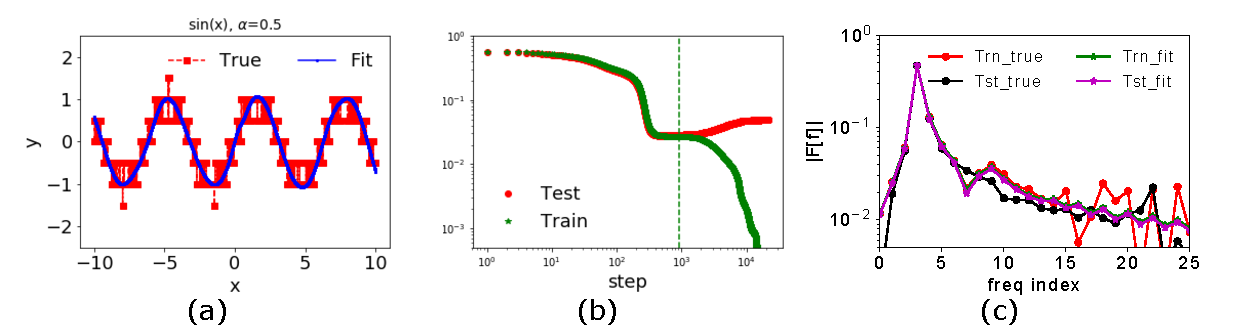
\includegraphics[width=0.98\linewidth]{figures/fprinciple/Fig3.pdf}
    \caption{图(a):使用DNN训练有噪声的正弦函数。图(b):损失函数分别在训练集测试集上的表现。图(c):训练集测试集在频率空间上的表现。}
    \label{fprinciple1}
\end{figure}


下面再举个更定量的例子,用来说明当正弦函数与其他高频函数叠加时,DNN会优先学习到更低频的部分,即正弦函数部分。从图\ref{fig:fpthree}可以看出,当DNN学习由函数$\sin (x)+\sin (5x)$生成的数据时,当epoch等于18000,神经网络可以学习处这个函数的大致趋势,并能较好的学习到$\sin (x)$的部分。只有当epoch继续增加,DNN才能学好这个函数各种高频的细节。
\begin{figure}[htbp!]
    \centering
    \subfigure[epoch:0]{
      \label{fig:subfig:onefunction} 
      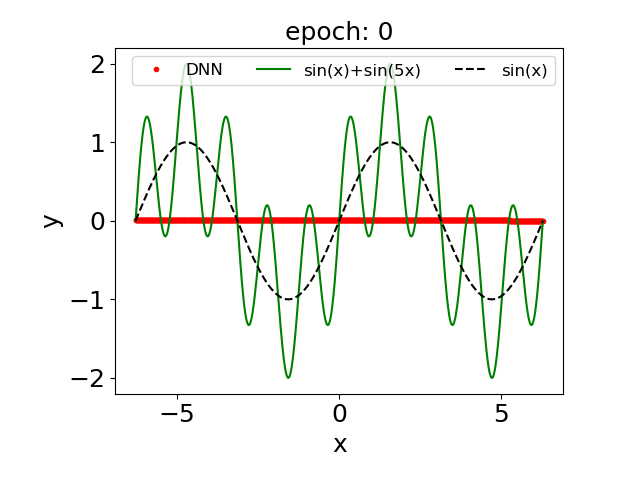
\includegraphics[scale=0.31]{figures/fprinciple/211210091512/ytestlow0.png}}
    % \hspace{0.5in} % 两图片之间的距离
    \subfigure[epoch:18000]{
      \label{fig:subfig:twofunction} 
      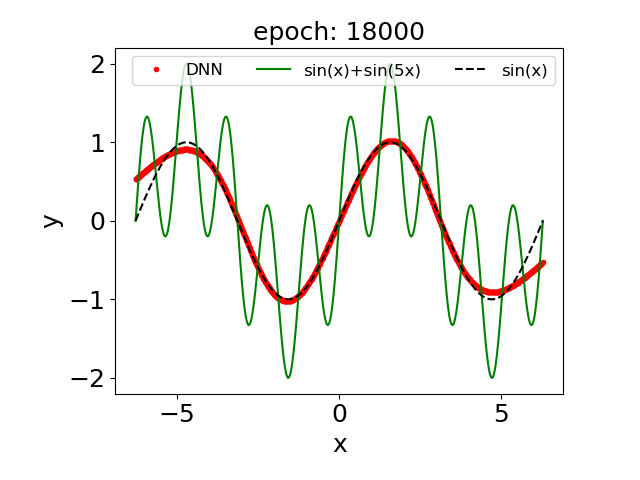
\includegraphics[scale=0.31]{figures/fprinciple/211210091512/ytestlow18000.png}}
      \subfigure[epoch:50000]{
      \label{fig:subfig:threefunction} 
      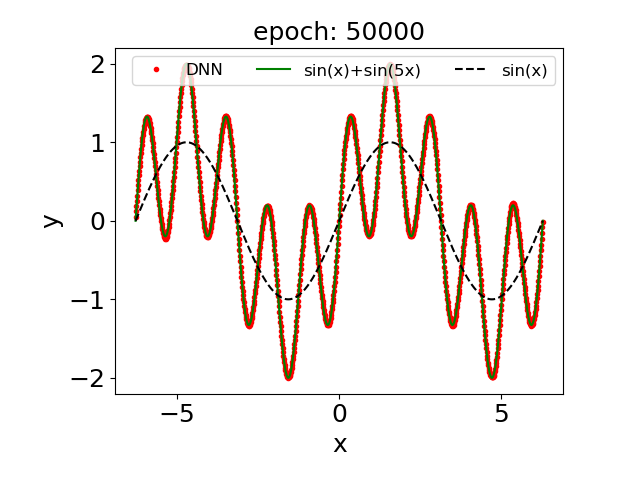
\includegraphics[scale=0.31]{figures/fprinciple/211210091512/ytestlow50000.png}}
    \caption{DNN学习函数$\sin (x)+\sin (5x)$,学习结果随epoch的变化,并与$\sin (x)$进行比较}
    \label{fig:fpthree}
  \end{figure}

从上面两个例子可以看出DNN确实可以先学习到低频部分,再学习到低频部分。那么,在学习中子共振的数据时,是不是只要我的epoch足够大,就一定能学好呢?答案显然不是,否则也没有发明PPSDNN算法的必要了。下面使用一个具体例子说明当频率稍微大一点时,传统DNN要学习好他们就必须付出极高的代价。在数值分析中,当插值函数的次数比较大时,会出现龙格现象。当使用DNN训练这类数据时,当参数数量和插值次数相仿时,就需要花费无穷大的epoch去训练他们,如图\ref{fig:fpfour}所示。有了f-principle的指导,在DNN中就不用再担龙格现象,并可以通过训练提前停止来避免过拟合。
\begin{figure}[htbp!]
    \centering
    \subfigure[epoch:250]{
      \label{onefunction} 
      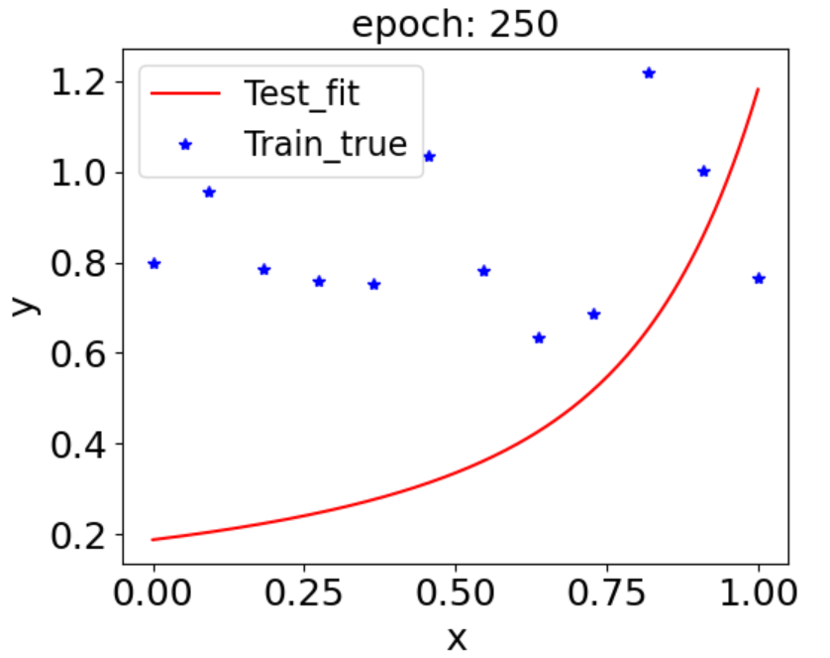
\includegraphics[scale=0.18]{figures/fprinciple/runge/e250.png}}
    % \hspace{0.5in} % 两图片之间的距离
    \subfigure[epoch:17500]{
      \label{twofunction} 
      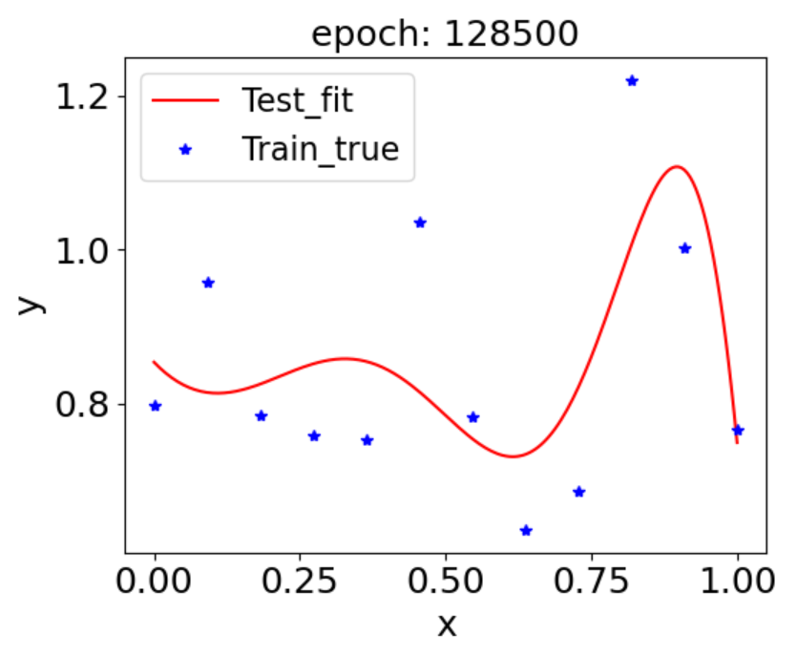
\includegraphics[scale=0.18]{figures/fprinciple/runge/e128500.png}}
      \subfigure[epoch:60750]{
      \label{threefunction} 
      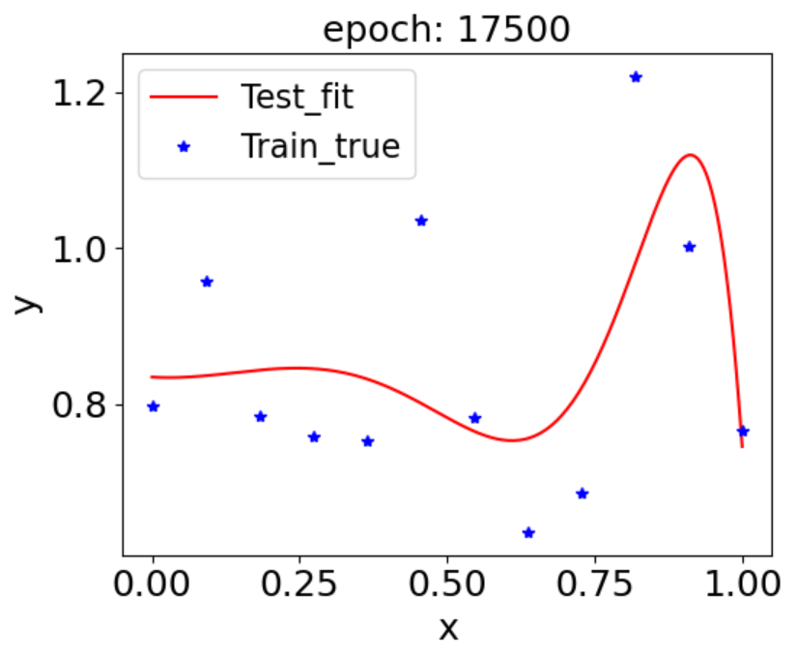
\includegraphics[scale=0.18]{figures/fprinciple/runge/e17500.png}}
      \subfigure[epoch:628500]{
      \label{fourfunction} 
      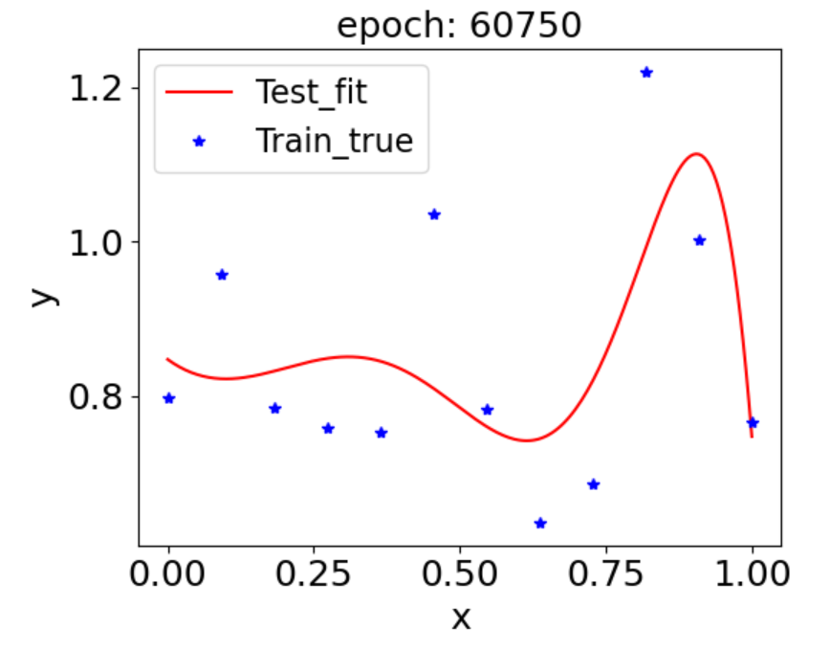
\includegraphics[scale=0.18]{figures/fprinciple/runge/e60750.png}}
    \caption{使用梯度下降学习11阶插值函数}
    \label{fig:fpfour}
  \end{figure}


f-principle 可以帮助我们理解DNN在不同问题上的优势和局限性,以及如何利用它们来设计更有效的算法。例如,在偏微分方程的数值求解中\cite{cai1996adaptive},可以结合DNN和传统迭代方法,先利用DNN快速收敛低频部分,再用传统迭代方法细化高频部分。

在中子共振核反应中,由于共振峰的存在,并根据第一章中的分析,在有限的高频共振能区中含有900多个共振峰,DNN并不能直接很好地应用于中子共振核反应的研究中。


使用DNN训练$^{235}\text{U}(n,f)$评价库数据,如图\ref{u235fp}所示,发现DNN只能较好的学习1/v能区和不可分辨能区的数据,对共振区的数据只能学习大致趋势,无法学到共振细节。为了验证DNN的训练效果不会随着epoch显著增加,可以画出损失函数的变化趋势,如图\ref{fig:u235fploss}所示,可以看出loss值在一定epoch之后不会再发生显著下降,即神经网络的学习效果不会再变好了。
\begin{figure}[htbp!]
    \centering
    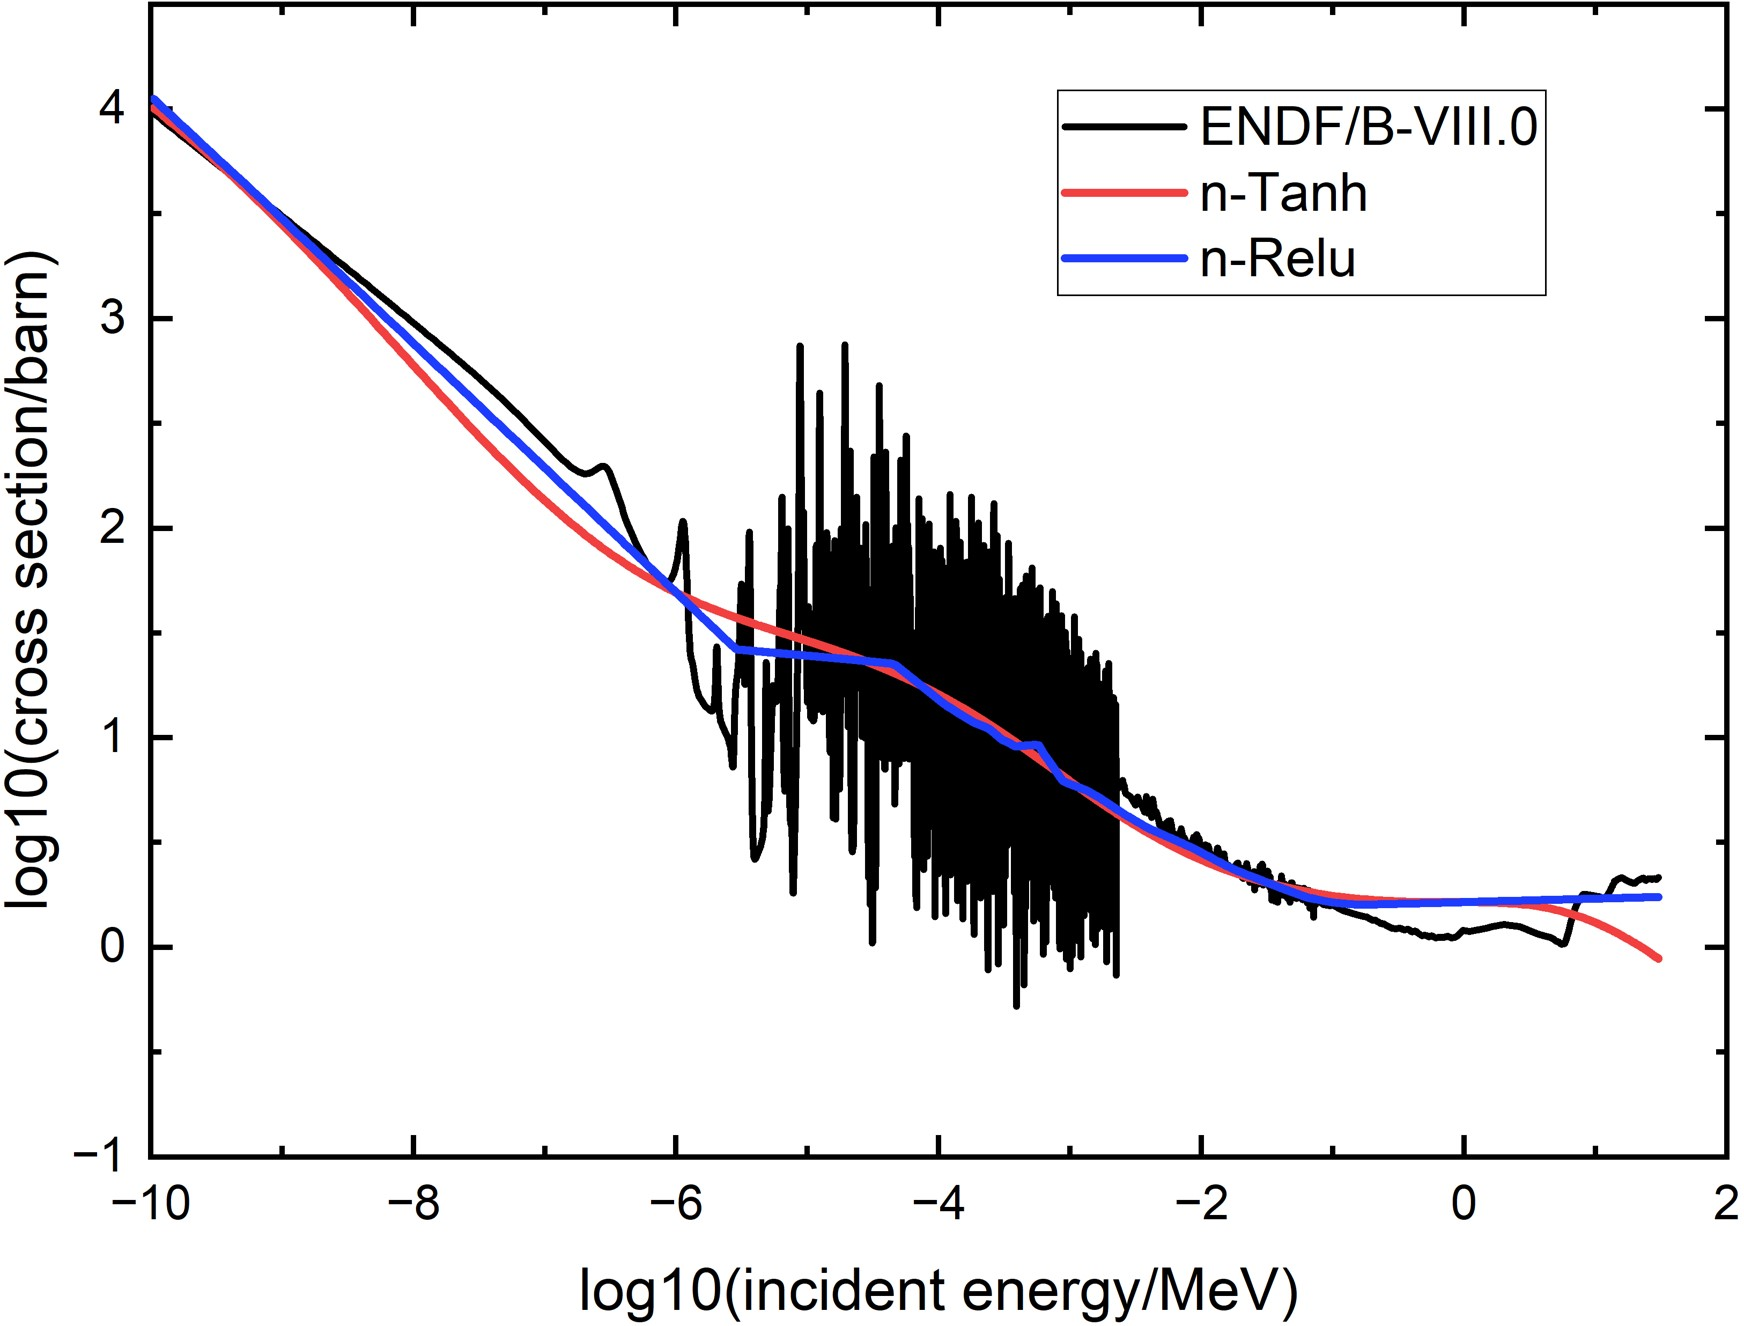
\includegraphics[width=0.76\linewidth]{figures/fprinciple/u235fp.jpg}
    \caption{使用tanh和relu激活函数分别对ENDF/B-VIII.0中$^{235}\text{U}(n,f)$反应截面进行学习}
    \label{u235fp}
\end{figure}
\begin{figure}[htbp!]
    \centering
    \subfigure[epoch:250]{
      \label{onefunu235relulossction} 
      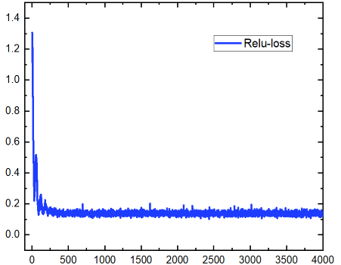
\includegraphics[scale=0.7]{figures/fprinciple/u235reluloss.png}}
    \hspace{0.5in} % 两图片之间的距离
    \subfigure[epoch:17500]{
      \label{u235tanhloss} 
      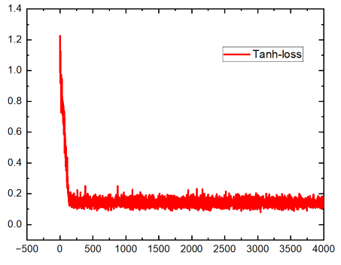
\includegraphics[scale=0.7]{figures/fprinciple/u235tanhloss.png}}
    \caption{不同激活函数下DNN的损失函数}
    \label{fig:u235fploss}
  \end{figure}


为解决DNN难以学习高频数据这个问题。本文中采用平行相移深度神经网
络模型\cite{cai2019phasednn}(Parallel Phase Shift Deep Neural Network,PPSDNN)。

\section{平行相移深度神经网络模型}

\subsection{模型及算法简介}
PPSDNN可以在训练过程中实现对函数的收敛,即同时逼近目标函数的低频和高频成分。PPSDNN利用了一个事实,即常见的DNN在训练时先收敛于低频范围,因此,它构造了一系列大小适中的DNN,并通过在频域上对训练数据进行相移操作,使得每个DNN能够逼近目标函数在特定范围内的高频内容。由于相移的作用,每个DNN都能够像在低频范围一样快速收敛。因此,PPSDNN能够将高频学习转化为低频学习,从而实现对函数的全部频域空间均匀学习和自适应训练。\cite{daubechies1992ten}
算法的大致思想是利用神经网络在训练过程中对低频成分的快速收敛,
通过相移技术将目标函数的高频成分转换为低频成分,然后用一系列并行的神经网络来近似不同频率范围的函数,
最后将这些神经网络的输出相加,从而得到目标函数的近似。

PPSDNN算法的基本思路如下:首先,将$f(x)$分解成各个频段函数的叠加。
\begin{equation}
f(x)=%
%TCIMACRO{\dsum \limits_{j=0}^{m}}%
%BeginExpansion
{\displaystyle\sum\limits_{j=0}^{m}}
%EndExpansion
f_{j}(x), \label{x-decomp}%
\end{equation}
其中,
\[
f_{j}(x)=\mathcal{F}^{-1}[\widehat{f_{j}}](x).
\]
谱区间为$[\omega _{j-1},\omega _{j+1}]$
设对于低频项,频域$k\in [-K_0,k_0]$,普通DNN方法可以给出很好的近似。
对于高频项,通过相移(phase shift)$r_{j}^{\text{shift}}(x_{i})=e^{i\omega_{j}x_{i}}r_{j}(x_{i})$,把高频数据转换成$[-K_0,k_0]$上的低频数据,进而使用DNN训练。将训练得到的结果再通过phase shift还原到高频部分。最后将训练的到的所有结果加起来就是总的训练结果。

PPSDNN算法可按如下几个模块逐步实现:
\begin{enumerate}
    \item 傅里叶变换和与尼奎斯特采样定理\cite{vaidyanathan2001generalizations}
    \item 单位分解定理(POU)
    \item B-样条函数
    \item 相移在频域空间中的实现
\end{enumerate}
\subsection{傅里叶变换与尼奎斯特采样定理}
傅里叶变换是把一个函数或一些离散数据从时域空间转换到频域空间,傅里叶逆变换则是从频域空间转换到时域空间\cite{xu2018understanding}。先考虑连续傅里叶变换(CFT)和连续傅里叶逆变换(ICFT),其公式为
    \begin{equation}
\mathcal{F}[g(x)](\xi)=\int_{-\infty}^{\infty} g(x) \mathrm{e}^{-2 \pi \mathrm{i} \xi x} \mathrm{~d} x, \quad \mathcal{F}^{-1}[\hat{g}(\xi)](x)=\int_{-\infty}^{\infty} \hat{g}(\xi) \mathrm{e}^{2 \pi \mathrm{i} \xi x} \mathrm{~d} \xi
\end{equation}
再考虑离散时域空间上的傅里叶变换(DTFT)及其逆变换
\begin{equation}
\begin{aligned}
& \mathcal{F}_{D T F T, \Delta}[g(x)](\xi)=\hat{g}_{D T F T}(\xi)=\sum_{j=-\infty}^{\infty} g(j \Delta) \mathrm{e}^{-2 \pi \mathrm{i} \xi j \Delta} \\
& \mathcal{F}_{D T F T, \Delta}^{-1}[\hat{g}(\xi)](j)=\Delta \cdot \int_{-\frac{1}{2 \Delta}}^{\frac{1}{2 \Delta}} \hat{g}_{D T F T}(\xi) \mathrm{e}^{2 \pi \mathrm{i} \xi j \Delta} \mathrm{d} \xi
\end{aligned}
\end{equation}
由于客观世界的数据往往是连续分布的,而我们认识的世界往往是通过离散的采样得到的数据。于是我们要尽可能在最大限度保留真实世界信息的情况下把CFT向DTFT转换。下面是转换公式的推导
\begin{equation}
\begin{aligned}
& \mathcal{F}_{D T F T, \Delta}[g(x)](\xi)=\sum_{j=-\infty}^{\infty} g(j \Delta) \mathrm{e}^{-2 \pi \mathrm{i} \xi j \Delta} \\
& =\sum_{j=-\infty}^{\infty} \int_{-\infty}^{\infty} \hat{g}\left(\xi^{\prime}\right) \mathrm{e}^{2 \pi \mathrm{i} \xi^{\prime} j \Delta} \mathrm{d} \xi^{\prime} \mathrm{e}^{-2 \pi \mathrm{i} \xi j \Delta} \\
& =\sum_{j=-\infty}^{\infty} \sum_{M=-\infty}^{\infty} \int_{\frac{M}{\Delta}-\frac{1}{2 \Delta}}^{\frac{M}{\Delta}+\frac{1}{2 \Delta}} \hat{g}\left(\xi^{\prime}\right) \mathrm{e}^{2 \pi \mathrm{i} \xi^{\prime} j \Delta} \mathrm{d} \xi^{\prime} \mathrm{e}^{-2 \pi \mathrm{i} \xi j \Delta} \\
& =\sum_{j=-\infty}^{\infty} \sum_{M=-\infty}^{\infty} \int_{-\frac{1}{2 \Delta}}^{\frac{1}{2 \Delta}} \hat{g}\left(\xi^{\prime}+\frac{M}{\Delta}\right) \mathrm{e}^{2 \pi \mathrm{i} \xi^{\prime} j \Delta} \mathrm{d} \xi^{\prime} \mathrm{e}^{-2 \pi \mathrm{i} \xi j \Delta} \\
&
\end{aligned}
\end{equation}
定义$\hat{h}\left(\xi^{\prime}\right)=\hat{g}\left(\xi^{\prime}+\frac{M}{\Delta}\right)$,得
\begin{equation}
\mathcal{F}_{D T F T, \Delta}[g(x)](\xi)=\frac{1}{\Delta} \sum_{M=-\infty}^{\infty} \sum_{j=-\infty}^{\infty}\left(\Delta \int_{-\frac{1}{2 \Delta}}^{\frac{1}{2 \Delta}} \hat{h}\left(\xi^{\prime}\right) \mathrm{e}^{2 \pi \mathrm{i} \xi^{\prime} j \Delta} \mathrm{d} \xi^{\prime}\right) \mathrm{e}^{-2 \pi \mathrm{i} \xi j \Delta}
\end{equation}
通过逆DTFT得
\begin{equation}
    \mathcal{F}_{DTFT,\Delta}[g(x)](\xi)=\dfrac{1}{\Delta}\sum\limits_{M=-\infty}^\infty\sum\limits_{j=-\infty}^\infty h(j\Delta)\mathrm{e}^{-2\pi i\xi j\Delta}.
\end{equation}
再通过DTFT得
\begin{equation}
    \begin{aligned}\mathcal{F}_{DTFT,\Delta}[g(x)](\xi)&=\frac{1}{\Delta}\sum_{M=-\infty}^\infty\bar{h}(\xi)\\ &=\frac{1}{\Delta}\sum_{M=-\infty}^\infty\hat{g}(\xi+\frac{M}{\Delta}).\end{aligned}
\end{equation}
在上式中,左边是离散时间中的采样,右边代表真是信号。其中,左边的$\xi \in [-\frac{1}{2\Delta },\frac{1}{2\Delta }  ]$。于是,可以得到尼奎斯特采样定理\cite{benedetto2001modern}。
\begin{thm}
一个有限带宽的连续信号可以被采样并且可以从它的采样中完美重构的条件为:采样频率大于真实频率的两倍。
\end{thm}
有了尼奎斯特采样定理,我们就能知道至少需要多少实验数据点才能学好中子共振截面的数据。

\subsection{单位分解定理}
在数学上,任意流形都能够表示成足够大的n维空间$\mathbb{R}^n$中某个曲面形式,而这可以用单位分解定理(Partition of Unity,POU)\cite{卓里奇2019数学分析}阐明。

\begin{thm}
设M是$C^{(k)}$光滑类的流形,X是M的子集。如果函数组$E= \{e_{\alpha},\alpha \in A\}$由$e_{\alpha} = C^{(k)}(M,\mathbb{R})$组成,且满足:

在X上$\sum_{e_{\alpha }\in E}^{}e_{\alpha }(x)\equiv 1 $。

那么,我们就说该函数组是集合X上的k阶光滑单位分解。
\end{thm}
在PPSDNN中,我们首先要将一个含有高频部分的目标函数f(x)通过傅里叶变换高频谱函数$\hat{f}(k)$,
再通过phase shift将频谱转换到$[-K_0,K_0]$的范围。下面考虑
$\widehat{f}(k)$上的支撑集,因为$\text{supp}\widehat{f}(k)=\{k \in \mathbb{R}|\widehat{f}(k)\ne 0\}$,
所以对给定的$\Delta k$,可以设$\widehat{f}(k)$上的支撑集为$\text{supp}\widehat{f}(k)\subset\lbrack-m\Delta k,m\Delta k].$。再将区间$[-m\Delta k,m\Delta k]$格点化,令$\omega _j = j \Delta k$,其中,$j = -m,...-1,0,1,...m$。下面考虑在区间$[-m\Delta k,m\Delta k]$上进行单位分解
\begin{equation}
1=%
%TCIMACRO{\dsum \limits_{j=0}^{m}}%
%BeginExpansion
{\displaystyle\sum\limits_{j=-m}^{m-1}}
%EndExpansion
\phi_{j}(k),\text{ }k\in\lbrack -m\Delta k,m\Delta k].\label{pou}%
\end{equation}

下面举几个满足单位分解定理的例子。
满足单位分解最简单的函数为$\phi _{j}(k)$:
\begin{equation}\label{eq:phij}
  \phi_j(k)=\phi(\frac{k-\omega_{j}}{\Delta k}) = \phi (\frac{k}{\Delta k}-j),
\end{equation}
其中,$\phi (k)$是区间$[-1,1)$上的特征函数,特征函数的形式为
\begin{equation}
    \phi (k) = \chi _{[0,1)}(k)= 
  \left\{\begin{matrix} 
  1,k \in[0,1)\\ 
  0,otherwise \\ 
\end{matrix}\right.  
\end{equation}
则对$\phi _j(k)$而言,$0\le \frac{k-\omega _j}{\Delta k}<1 $时,即$j\Delta k\le k<(j+1)\Delta k$时为1,其余区间为0,即
\begin{equation}
    \phi _j(k)= \left\{\begin{matrix} 
  1,k \in[j\Delta k,(j+1)\Delta k)\\ 
  0,otherwise \\ 
\end{matrix}\right.
\end{equation}
这样的2m个函数$\phi_{-m}(k),\phi_{-m+1}(k),...\phi_{0}(k),...\phi_{m-2}(k),\phi_{m-1}(k),$
对应的值为1的非零区间为$[-m\Delta k,(-m+1)\Delta k),[-(m+1)\Delta k,(-m+2)\Delta k),...,[(m-2)\Delta k,(m-1)\Delta k),[(m-2)\Delta k,(m-1)\Delta k)$。因此,当$-m\Delta k\le  k\le m\Delta k$时,必落在某个区间,使某个$\phi _j(k)=1$,其余的$\phi _j(k)=0$,即$\sum_{j=-m }^{m-1}\phi_j(k) = 1$。因此$\phi_j(k)$满足单位分解定理(POU)。下面计算$\phi (k) = \chi _{[0,1)}(k)$的逆傅里叶变换,我们用符号$\vee$表示。
\begin{equation}\label{eq:invfphi}
  \phi^{\vee}(x) = \frac{1}{\sqrt{2\pi} } \int_{0}^{1} dke^{ikx}=\frac{e^{\frac{ix}{2}(e^{\frac{ix}{2} }-e^{-\frac{ix}{2} }) }}{ix\sqrt{2\pi}}
  = \frac{1}{\sqrt{2\pi}}e^{i\frac{x}{2}}\frac{\sin x/2}{x/2}.
\end{equation}

 虽然特征函数可以构造出满足单位分解的函数,但特征函数是分段函数,且不够光滑。下面我们使用B-样条函数构造满足单位分解的函数,这样的函数满足连续且光滑的条件。



\subsection{B-样条函数}
B-样条函数\cite{prochazkova2005derivative}是基于特征函数迭代递推得到的,它和特征函数相比具有更连续更光滑的性质。采用如下卷积迭代的方式可以定义B-样条函数
\begin{equation}
    \left\{\begin{matrix} 
&B_{1}(k)=\chi_{\lbrack0,1)}(k),\\
&B_{m}(k)=B_{m-1}(k)\ast\chi_{\lbrack0,1)}(k),m=2,\cdots.\label{b-spline}%
\end{matrix}\right. 
\end{equation}
这种递推关系式也可以写成
\begin{equation}
    B_{m}(k)=\underbrace{B_1(k) * B_{1}(k) * \cdots * B_{1}(k)}_{m \text{个}}
\end{equation}
其中$*$代表卷积,即$(f * g)(t) \stackrel{\text { def }}{=} \int_{\mathbb{R}^{n}} f(\tau) g(t-\tau) d \tau$
可以用归纳法证明
\begin{equation}
    supp B_{m}(k)=[0,m)
\end{equation}
下面,分别举m=2和m=3的例子来说明B-样条函数的支撑集以及它的连续性和光滑性。

当m=2时
\begin{equation*}
    B_{2}(k)=B_{1}(k)\star B_{1}(k)=\int_{-\infty}^{\infty}B_{1}(k-\lambda)B_{1}(\lambda)d\lambda=
\int_{0}^{1}B_{1}(k-\lambda)d\lambda
\end{equation*}
其中
\begin{equation*}
    \left\{\begin{matrix} 
0 \le \lambda <1,\\
0\le k-\lambda <1
\end{matrix}\right. 
\Rightarrow 0\le k <2
\end{equation*}
于是不难看出
\begin{equation}
    supp B_2(k)=[0,2)
\end{equation}
通过积分,不难得出
\begin{equation}
B_2(k)=
    \left\{\begin{matrix} 
k,0\le k<1\\
2-k,1\le k<2\\
0,otherwise
\end{matrix}\right. 
\end{equation}
可以看出,$B_2(k)$虽然连续,但不光滑。如图\ref{B2}
\begin{figure}[htbp]
    \centering
    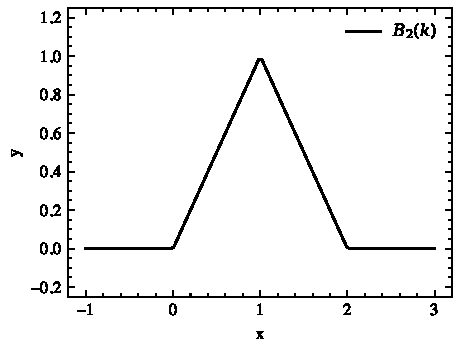
\includegraphics[width=0.76\linewidth]{figures/B-splin/B2.pdf}
    \caption{2阶B样条函数}
    \label{B2}
\end{figure}

当m=3时,同理可得
\begin{equation*}
    B_{3}(k)=B_{2}(k)\star B_{1}(k)=\int_{-\infty}^{\infty}B_{2}(k-\lambda)B_{1}(\lambda)d\lambda=
\int_{0}^{1}B_{2}(k-\lambda)d\lambda
\end{equation*}
且不难看出
\begin{equation}
    supp B_3(k)=[0,3)
\end{equation}
通过积分,不难得出
\begin{equation}
B_3(k)=
    \left\{\begin{matrix} 
\frac{1}{2}k^2 ,0\le k<1\\
\frac{1}{2}+(k-1)-(k-1)^2 ,1\le k<2\\
\frac{1}{2}-(k-2)+\frac{1}{2} (k-2)^2 ,2\le k<3\\
0,otherwise
\end{matrix}\right. 
\end{equation}
此时,在k=1和k=2处,$B_3(k)$不仅连续,而且光滑(一阶导数连续)。如图\ref{B3}
\begin{figure}[htbp]
    \centering
    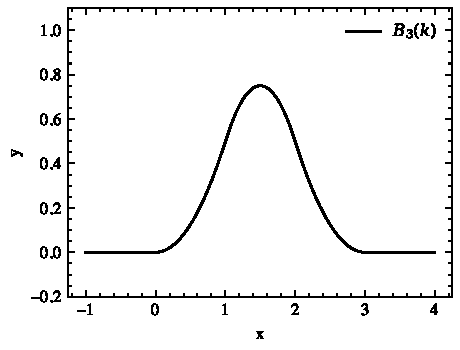
\includegraphics[width=0.76\linewidth]{figures/B-splin/B3.pdf}
    \caption{3阶B样条函数}
    \label{B3}
\end{figure}

于是,可以整理出B-样条函数的诸多性质,如
\begin{enumerate}
    \item $\text{supp} B_m(k)=[0,m)$
    
    证明:采用归纳法。

    在上文中,我们通过计算m=1,m=2,m=3给出了具体几个常用特例的证明。下面,采用数学归纳法给出普式的m的证明。

    设$\text{supp} B_m(k)=[0,m)$,则
    \begin{equation*}
    B_{m+1}(k)=B_{m}(k)\star B_{1}(k)=\int_{-\infty}^{\infty}B_{m}(k-\lambda)B_{1}(\lambda)d\lambda=
\int_{0}^{1}B_{m}(k-\lambda)d\lambda
\end{equation*}
其中
\begin{equation*}
    \left\{\begin{matrix} 
0 \le \lambda <1,\\
0\le k-\lambda <m
\end{matrix}\right. 
\Rightarrow 0\le k <m+1
\end{equation*}
于是,$\text{supp} B_m(k)=[0,m)$,证毕。
    \item $B_m(k)$的逆傅里叶变换
    
    通过卷积定理:
    \begin{equation}
        \left\{\begin{matrix} 
& \mathcal{F} [f(x)*g(x)]= \hat{f}(k)\hat{g}(k)  \\
& \mathcal{F}[f(x)g(x)] = \hat{f}(k)*\hat{g}(k)\Rightarrow f(x)g(x) = \mathcal{F}^{-1}[\hat{f}(k)*\hat{g}(k)] \\
\end{matrix}\right. 
    \end{equation}
其中,为了符号书写方便,把傅里叶逆变换定义为$\mathcal{F[\cdot ]}$。

这样,$B_m(k)$的逆傅里叶变换,记为$B_m^{\vee}(k)$,有
\begin{align}
B_{m}^{\vee}(x)  &  =\left(  B_{1}^{\vee}(x)\right)  ^{m}=\left(  \frac
{1}{\sqrt{2\pi}}e^{i\frac{x}{2}}\frac{\sin\frac{x}{2}}{\frac{x}{2}}\right)
^{m}\nonumber\\
&  =\frac{e^{i\frac{mx}{2}}}{\left(  2\pi\right)  ^{m/2}}\left(  \frac
{\sin\frac{x}{2}}{\frac{x}{2}}\right)  ^{m}.
\end{align}
\end{enumerate}
下面将在“相移在频域空间中的实现”部分介绍如何使用B-样条函数构造满足单位分解的函数。


\subsection{相移在频域空间中的实现}
我们以四次B-样条函数为例,构造满足单位分解的函数。首先,令$\phi(k)=B_{4}(k+2)$,接着构造
\begin{equation}
    \phi_j(k)=\phi(k/\Delta k-j)=B_4(\frac{k}{\Delta k}+2-j)
\end{equation}

可以证明,该函数满足单位分解。将$\phi_j(k)$做傅里叶逆变换,得到频率选择函数(frequency selection kernel),为了得到$\phi_{j}^{\vee}(x)$,我们先求$\phi^{\vee}(x)$,得
\begin{equation}
    \begin{aligned} 
        &\phi^{\vee}(x) =\frac{1}{\sqrt[]{2\pi } }\int_{\mathcal{R} }^{}  B_4(k+2)e^{ikx}dk \\
      &\overset{令k+2=k'}{=} \frac{1}{\sqrt[]{2\pi } }\int_{\mathcal{R} }^{}dk'B_4(k')e^{ik'x}e^{-2ix}\\
      &=B_4^{\vee } (x)e^{-2ix}=\frac{1}{(2\pi)^2}(\frac{\sin{x/2}}{x/2})^4
      \end{aligned}
\end{equation}
下面计算$\phi_j(k)$的傅里叶逆变换,的
\begin{equation}
    \begin{aligned} 
        & \phi_{j}^{\vee}(x)=\frac{1}{\sqrt[]{2\pi } }\int_{\mathcal{R} }^{}dk\phi(\frac{k}{\Delta k}-j )e^{ikx}  \\
       &\overset{k'=k/\Delta k}{=}\frac{1}{\sqrt[]{2\pi } }\int_{\mathcal{R} }^{}  (\Delta k)dk'\phi (k'-j)e^{ik'\Delta kx}  \\
       &\overset{k''=k'-j}{=}\frac{1}{\sqrt[]{2\pi } }\int_{\mathcal{R} }^{}  (\Delta k)dk''\phi (k'')e^{i(k''+j)\Delta kx}\\
       &=\Delta ke^{-ij\Delta kx}\phi^{\vee}(\Delta kx)=K_0e^{-ijK_{0}x}%
       \phi^{\vee}(K_{0}x),
       \end{aligned}.
\end{equation}
下面求$\phi_{j}(k)$的支撑集。由前面的定义和结论,显然,有$supp\phi _j(k)=supp\mathcal{F}[\phi_{j}^{\vee}(x)]$。于是,根据$0\le \frac{k}{\Delta k}+2-j<4$得,$\omega_{j-2}\le k<\omega_{j+2}$,即
\begin{equation}
    supp\mathcal{F}[\phi_{j}^{\vee}(x)]\subset\lbrack\omega_{j-2}, \omega_{j+2}].
\end{equation}

同样,可以证明B-样条函数满足单位分解性质。
前面假设了低频空间为$k\in [-m\Delta k,\Delta k]$,通过移项得$-m\le \frac{k}{\Delta k}\le m$。又$0\le \frac{k}{\Delta k}+2-j<4$,移项得$-2+\frac{k}{\Delta k}<j\le 2+\frac{k}{\Delta k}$。不难得出
\begin{equation*}
    -m-2<j\le m+2
\end{equation*}
因此,j实际的范围是$j = -m-1,-m,...,0,...,m+1,m+2$。
因此,可以证明$\phi_{j}(k)$满足单位分解。
\begin{equation}\label{eq:sum1C4}
  \sum_{j=-m-1}^{m+2}\phi_j(k) = 1 ,\quad \forall k\in [-m\Delta k, m\Delta k].
\end{equation}
在实际我们选择POU函数时,对于$\sum_{j}^{}\phi_j(k) = 1$,j的具体范围取决于:

    1) k的范围;
    2) 样条函数的选取;
    3) 样条函数的平移量。


然后,在POU的基础上,我们对想要分解的函数f(x)做傅里叶展开(傅里叶逆变换),即
\begin{equation}
    f(x) = \frac{1}{\sqrt{2\pi}}\int_{\mathcal{R} }^{}dk\hat{f}(x)e^{ikx}  \label{Ff}
\end{equation}
其中,$\hat{f}(k)$可以利用POU的性质分解为
\begin{equation}
\widehat{f}(k)=%
%TCIMACRO{\dsum \limits_{j=0}^{m}}%
%BeginExpansion
{\displaystyle\sum\limits_{j=-m}^{m-1}}
%EndExpansion
\phi_{j}(k)\widehat{f}(k)\triangleq%
%TCIMACRO{\dsum \limits_{j=0}^{m}}%
%BeginExpansion
{\displaystyle\sum\limits_{j=-m}^{m-1}}
%EndExpansion
\widehat{f_{j}}(k). \label{k-decomp}%
\end{equation}
相应的,把\ref{k-decomp}式代入\ref{Ff}式,可以在时域空间里将f(x)做分解
\begin{equation}
f(x)=%
%TCIMACRO{\dsum \limits_{j=0}^{m}}%
%BeginExpansion
{\displaystyle\sum\limits_{j=0}^{m}}
%EndExpansion
f_{j}(x), \label{x-decomp}%
\end{equation}
其中,
\[
f_{j}(x)=\mathcal{F}^{-1}[\widehat{f_{j}}](x).
\]
根据POU,
\begin{equation*}
    f_{j}(x) = \frac{1}{\sqrt{2\pi}}\int_{\omega _j }^{\omega_{j+1}}dk\hat{f_j}(k)e^{ikx}=\\
    \frac{1}{\sqrt{2\pi}}\int_{\omega _j }^{\omega_{j+1}}dk\phi_j(k)\hat{f}(k)e^{ikx}=\mathcal{F}^{-1}[\phi_j \hat{f}]
\end{equation*}
由卷积定理,$\mathcal{F}[f(x)*g(x)] = \hat{f}(k)\hat{g}(k)$,即$f(x)*g(x) = \mathcal{F}^{-1}[\hat{f}(k)\hat{g}(k)]$。
所以,
\begin{equation}
    f_j(x) = \phi_j^{\vee}(x)*f(x)=\int_{-\infty }^{\infty} \phi _j^{\vee}(x-s)f(s)ds
\end{equation}
从上式可以看出,$\phi_j^{\vee}(x)$通过卷积作用到f(x)上得到频率空间为$[\omega_j,\omega_{j+1}]=[j\Delta k,(j+1)\Delta]=[jK_0,(j+1)K_0]$的分量。$f_j(x)$在此称为频率选择函数(frequency selection kernal)。

基于频率选择函数,就可以实现平行相移。
设当函数f(x)通过傅里叶变换转换到频域空间,且$|k|<K_0$时,函数处于低频,DNN可以很好的训练f(x)的低频量。对f(x)的高频量$f_j(x)$,我们可以通过乘一个相移因子,将其转换到$|k|<K_0$的区域,具体形式为:
\begin{equation}
    f_j^{\text{shift}}(x) = e^{i\omega_jx}f_j(x)
\end{equation}
下面分析$f_j^{\text{shift}}(x)$的频率范围,这里的推导需要用到$\delta$函数的性质。
\begin{equation}
    f_j^{\text{shift}}(k) = \hat{f}_j(k-\omega_j)
\end{equation}
如果$f_j(k)$的支撑集为$[\omega_j,\omega_{j+1}]$,则$supp[f_j^{\text{shift}}(k)]\subset [0,K_0]$。于是,我们通过phase shift将f(x)的高频部分转换到了低频部分。于是可以将低频部分使用DNN去训练。下面介绍PPSDNN的算法流程。


\section{算法流程}
首先,给定一个要用来训练的目标函数f(x)。我们使用DNN$T_{\star}(x,\theta^{(n_{0}%
)}),x\in R,$去逼近它。
\begin{equation}
T_{\star}(x,\theta^{(n_{0})})=f_{\text{DNN}}(x)\approx f(x),\label{f1(x)}%
\end{equation}
$f_{\text{DNN}}(x)$和f(x)各自对应的低频部分可以拟合的很好,但高频部分仍然会有差距。于是定义余项$r(x)=f(x)-f_{\text{DNN}}(x)$,并规定低频区域
\begin{equation}
\left\vert \mathcal{F}[r](k)\right\vert \ll1\text{ for }\left\vert
k\right\vert <K_{0},
\end{equation}
这样,才能确保
\begin{equation}
\mathcal{F}[f](k)\approx\mathcal{F}[f_{\text{DNN}}(x)](k),\quad k\in
(-K_{0},K_{0}).\label{eq:1psdnn}%
\end{equation}

如果精确知道r(x),则$f(x) = r(x) + f_{\text{DNN}}(x)$。为尽量精确求得r(x),首先将r(x)分解,
\begin{equation}
r(x)=%
%TCIMACRO{\dsum \limits_{j=0}^{m}}%
%BeginExpansion
{\displaystyle\sum\limits_{j=0}^{m}}
%EndExpansion
r_{j}(x),
\end{equation}
其中
\begin{equation}
r_{j}(x)=\mathcal{F}^{-1}[\widehat{r_{j}}(k)]=\mathcal{F}^{-1}[\phi
_{j}(k)\widehat{r}(k)](x).\label{rj(x)}%
\end{equation}
训练数据$\{r_{j}(x_{i})\}_{i=1}^{N}$可以由\ref{rj(x)}式计算得到,在时域空间上,这些离散数据点可以通过下面的卷积公式得到
\begin{align}
r_{j}(x_{i}) &  =\phi_{j}^{\vee}\ast r(x_{i})=\int_{-\infty}^{\infty}\phi
_{j}^{\vee}(x_{i}-s)r(s)ds\nonumber\\
&  \approx\frac{2\delta}{N_{s}}%
%TCIMACRO{\dsum \limits_{x_{s}\in(x_{i}-\delta,x_{i}+\delta)}}%
%BeginExpansion
{\displaystyle\sum\limits_{x_{s}\in(x_{i}-\delta,x_{i}+\delta)}}
%EndExpansion
\phi_{j}^{\vee}(x_{i}-x_{s})r(x_{s}),\label{convol}%
\end{align}
取相应的频率选择核$r_{j}(x)$,可以将$\phi_j(x)$的频率范围,即支撑集调整到$[\omega_{j-1,}\omega_{j+1}]$。


接下来对$r_j(x)$作phase shift。
\begin{equation}
r_{j}^{\text{shift}}(x)=e^{i\omega_jx}r_j(x)=\mathcal{F}^{-1}\left[  \widehat{r_{j}}(k-\omega
_{j})\right]  (x),\label{rjshift}%
\end{equation}
则$r_{j}^{\text{shift}}(x)$的支撑集在$[-K_0,K_0]$之间。所以$r_{j}^{\text{shift}}(x)$属于低频部分,所以它可以由DNN相对精确且快速地得到。即
\begin{equation}
T_{j}(x,\theta^{(n_{0})})\ \approx r_{j}^{\text{shift}}(x),0\leq j\leq m,
\end{equation}
相应的$r_j(x)$为
\begin{equation}
r_{j}(x)\approx e^{-i\omega_{j}x}T_{j}(x,\theta^{(n_{0})}).
\end{equation}
于是
\begin{equation}
r(x)\approx%
%TCIMACRO{\dsum \limits_{j=0}^{m}}%
%BeginExpansion
{\displaystyle\sum\limits_{j=0}^{m}}
%EndExpansion
e^{-i\omega_{j}x}T_{j}(x,\theta^{(n_{0})}).
\end{equation}
最终,我们得到
\begin{equation}
f(x) \approx f_{\text{DNN}}(x)+%
%TCIMACRO{\dsum \limits_{j=0}^{m}}%
%BeginExpansion
{\displaystyle\sum\limits_{j=0}^{m}}
%EndExpansion
e^{-i\omega_{j}x}T_{j}(x,\theta^{(n_{0})}). \label{DNNupdate}%
\end{equation}
以上便是PPSDNN的全部算法。本算法可以使用python语言实现,用pytorch\cite{ketkar2021introduction}编写。

pytorch提供了专门的fft包用于计算傅立叶变换,傅立叶变换是fft,逆变换是ifft。另外,pytorch还提供了一个非常有用的函数:fftfreq,它可以得到离散傅立叶变换的采样频率。
特别值得关注的是,当$T(x)$是复函数时,可以用傅立叶级数展开:
\begin{equation}\label{}
    T(x)=\sum_{m=1}^{M} e^{i \omega_{m} x} T_{m}(x)
\end{equation}
在本工作中,$T(x)$是实函数,它可以用下面的级数作展开:
\begin{equation}\label{}
    T(x)=\sum_{m=1}^{M} A_{m} \cos \left(\omega_{m} x\right)+B_{m} \sin \left(\omega_{m} x\right).
\end{equation}
其中$\omega_{m}$是相移频率。
在pytorch中,通常用torch.nn, torch.nn.Module等模块来定义神经网络模型和神经网络的前向传播。使用torch.optim指定DNN的优化器。
使用torch.autograd.grad, optimizer.step和backward函数进行神经网络的反向传播过程。

算法大致流程如图\ref{ppsdnnchart}所示:
\begin{figure}[htbp]
    \centering
    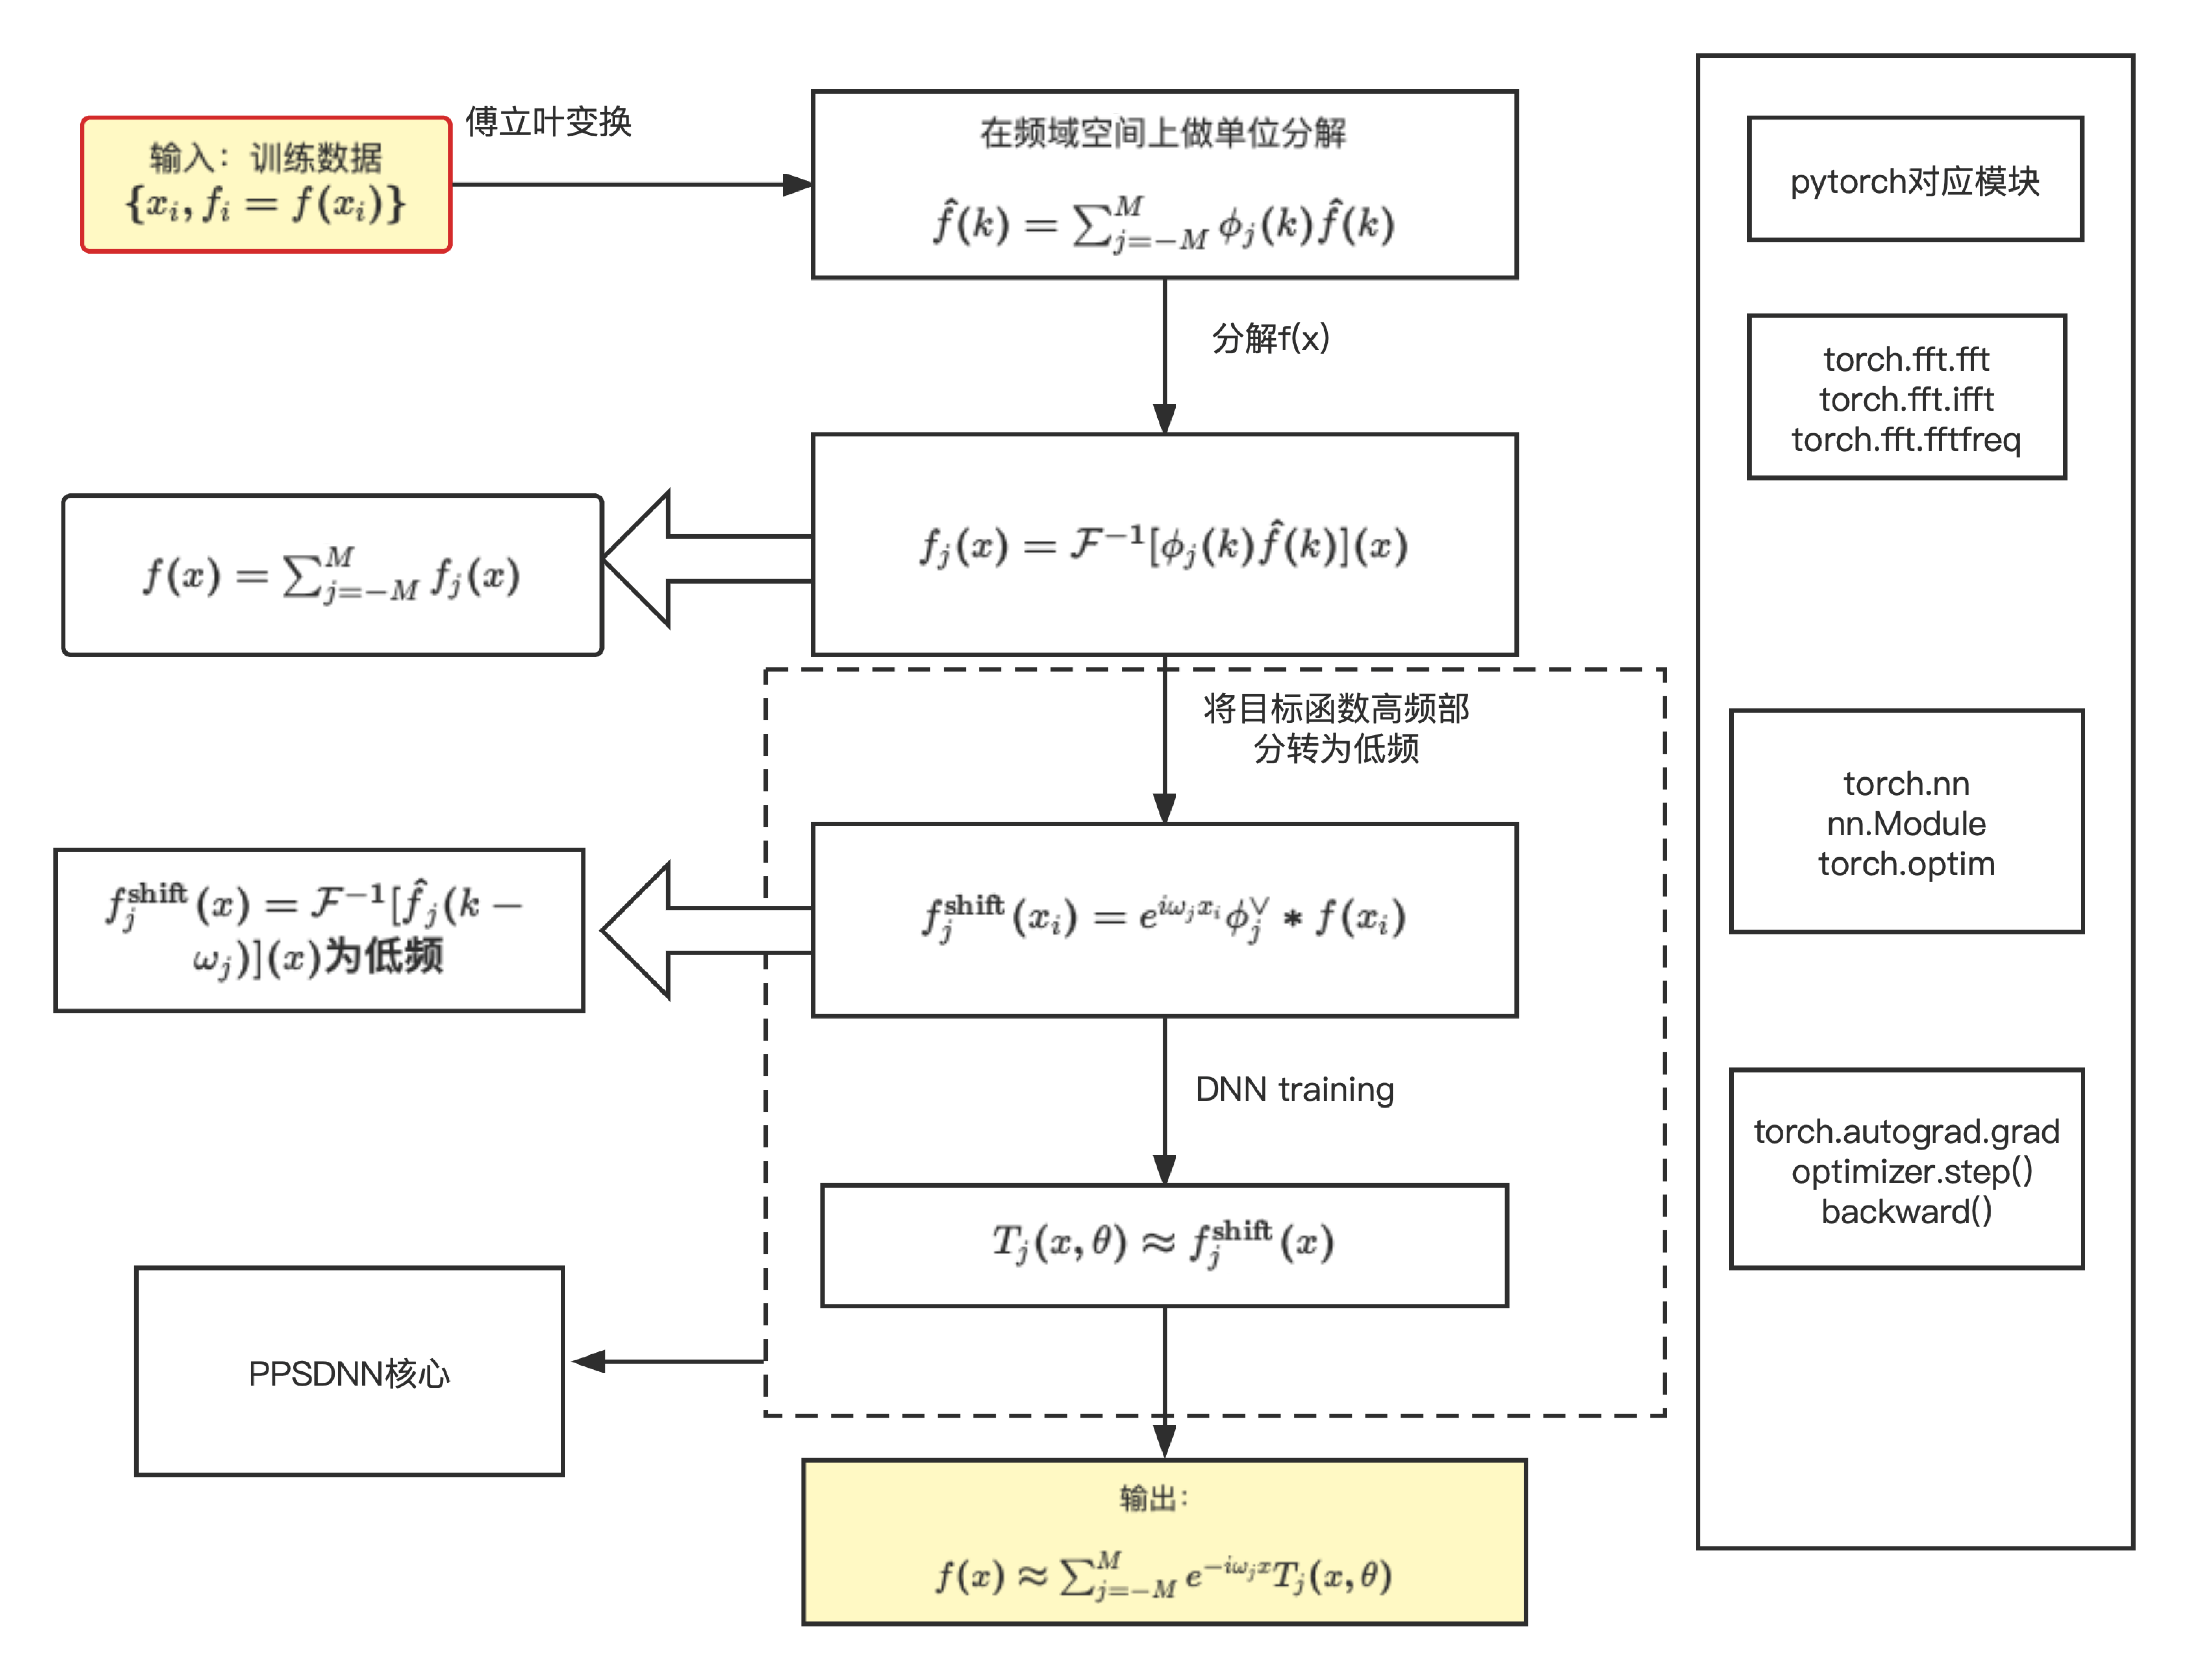
\includegraphics[width=0.95\linewidth]{figures/ppsdnnchart.pdf}
    \caption{PPSDNN算法流程图}
    \label{ppsdnnchart}
\end{figure}



